\documentclass[12pt]{article}
\usepackage{graphicx}
\usepackage{subcaption}
\usepackage{amssymb}
\usepackage{amsmath}
\graphicspath{ {images/} }
\usepackage[margin=1in]{geometry}
\usepackage{float}
\title{Cable Project}
\author{Darice, Elise, Sarah}


\begin{document}
\maketitle




 
 When $\lambda<0$, if $c^2\geq4(1+\lambda)$, then $F(\xi)=Ae^{\frac{1}{2}\big(-c+\sqrt{c^2+4(1+\lambda)}\big)\xi}+Be^{-\frac{1}{2}\big(c+\sqrt{c^2+4(1+\lambda)}\big)\xi}$. The boundary condition in equation \ref{psiBC} requires that $B=0$ when $V>\theta$ and that $A=0$ when $V<\theta$. \\
 
 
 ???-->
 When $\lambda<0$, if $c^2<|4(1+\lambda)|$, then $F(\xi)=e^{\frac{-c}{2}}\Big(C cos\big(\frac{\sqrt{|c^2+4(1+\lambda)|}}{2}\xi\big)+D sin\big(\frac{\sqrt{|c^2+4(1+\lambda)|}}{2}\xi\big)\Big)$.
 
 
$v(x,t)=V(\xi)+\epsilon\psi(\xi,t)$






\subsection{Stability of the Traveling Front Solutions}
Now that we have found the traveling front solutions, it is important to understand their stability using linear stability analysis. Consider the solution $v(x,t)=V(\xi)+\epsilon\psi(\xi,t)$, where $0 < \epsilon <<1$ and $\psi(\xi,t)$ represents a small perturbation to the traveling wave solution, $V(\xi)$. The goal of the linear stability analysis is to understand how $\psi(\xi,t)$ behaves over time. Recall the governing partial differential equation
\begin{equation}
\label{uh}
\frac{\partial v}{\partial t}=\frac{\partial ^2 v}{\partial x^2}-v+H(v-\theta)
\end{equation}
\\
The chain rule allows us to obtain the following partial derivatives of $v(x,t)=V(\xi)+\epsilon\psi(\xi,t)$.

$$\frac{\partial v}{\partial t}=\frac{\partial\xi}{\partial t}\frac{dV}{d\xi}+\epsilon(\frac{\partial \psi}{\partial \xi}\frac{\partial \xi}{\partial t}+\frac{\partial \psi}{\partial t}) = -c\frac{dV}{d\xi}+\epsilon(-c\frac{\partial \psi}{\partial \xi}+\frac{\partial \psi}{\partial t})$$

$$\frac{\partial v}{\partial x}=\frac{\partial \xi}{\partial x}\frac{dV}{d\xi}+\epsilon\frac{\partial\xi}{\partial x}\frac{\partial\psi}{\partial\xi} = \frac{dV}{d\xi}+\epsilon\frac{\partial\psi}{\partial\xi}$$

$$\frac{\partial^2 v}{\partial x^2}=\frac{\partial \xi}{\partial x}\frac{d^2V}{d\xi^2}+\epsilon\frac{\partial^2\psi}{\partial\xi^2}\frac{\partial \xi}{\partial x} = \frac{d^2V}{d\xi^2}+\epsilon\frac{\partial^2\psi}{\partial\xi^2}$$
Equation (\ref{uh}) is rewritten as 
\begin{equation}
\label{frewritten}
-c\frac{dV(\xi)}{d\xi}+\epsilon(-c\frac{\partial \psi(\xi,t)}{\partial \xi}+\frac{\partial \psi(\xi,t)}{\partial t})=\frac{d^2V(\xi)}{d\xi^2}+\epsilon\frac{\partial^2\psi(\xi,t)}{\partial\xi^2}+f(V(\xi)+\epsilon\psi(\xi,t))
\end{equation}
Analysis of equation (\ref{frewritten}) can be simplified by using the Taylor expansion of $f\big(V(\xi)+\epsilon\psi(\xi,t)\big)$ with respect to $V(\xi)$, and discounting $O(\epsilon ^2)$ terms.

$$f\big(V+\epsilon\psi \big) \approx f(V) + \frac{\partial f(V)}{\partial V}\epsilon\psi = -V +\mathcal{H}(V-\theta) - \epsilon\psi + \delta(V-\theta)\epsilon\psi $$
Equation \ref{frewritten} becomes
$$-c\frac{dV}{d\xi}+\epsilon(-c\frac{\partial \psi}{\partial \xi}+\frac{\partial \psi}{\partial t})= 
\frac{d^2V}{d\xi^2}+\epsilon\frac{\partial^2\psi}{\partial\xi^2}-V+H(V-\theta)+\epsilon\psi\big(-1+\delta(V-\theta)\big)$$
Look at the terms involving $\psi$ and $\epsilon$ to analyze the long term behavior of the disturbance. The partial differential equation that models the behavior of the perturbation is

\begin{equation} \label{pde_nh}
\frac{\partial \psi}{\partial t} = c \frac{\partial^2\psi}{\partial\xi^2} + \frac{\partial\psi}{\partial\xi} - (1 - \delta(V-\theta))\psi
\end{equation} 


\subsection{Separation of Variables}

This equation can be solved using separation of variables, where solutions have the form of $\psi(\xi,t)=S(\xi)T(t)\neq0$.

$$ \frac{1}{T}\frac{\partial T}{\partial t} = \frac{1}{S}\frac{\partial^2S}{\partial\xi^2} + \frac{c}{S}\frac{\partial S}{\partial\xi} - 1 + \delta(V-\theta)= \lambda $$
Before proceeding with the analysis, we need to define the boundary conditions. Recall that the boundary condition $\lim_{x\to\pm\infty} \frac{\partial v(x,t)}{\partial x}=0$ is necessary to ensure a physically realistic solution. Because we previously imposed the boundary condition that $\lim_{\xi\to\pm\infty} \frac{dV}{d\xi}=0$, it must also be true that 

$$\lim_{x\to\pm\infty} \frac{\partial \big(V(\xi)+\epsilon\psi(\xi,t)\big)}{\partial x} = \lim_{\xi\to\pm\infty} \frac{dV}{d\xi}+\lim_{\xi\to\pm\infty} \epsilon\frac{\partial\psi}{\partial\xi}=0 \implies \lim_{\xi\to\pm\infty}\frac{d\psi}{d\xi}=0 $$
The time-dependent equation is a homogeneous ODE with the following solutions, where $a\in\mathbb{R}$.
\begin{equation} \label{timeeq}
\frac{1}{T}\frac{dT}{dt} = \lambda \implies \int\frac{dT}{T} = \int\lambda dt \implies T(t)=ae^{\lambda t}
\end{equation}
For the spatial dependence, we split the domain of the equation into three regions, depending on the value of $\delta(V(\xi)-\theta)$, with the boundary condition that $\lim_{\xi \to \pm \infty}\psi = 0$:

Region 1: $\xi < 0$ and $\delta(V(\xi)-\theta) = 0$

Region 2: $\xi > 0$ and $\delta(V(\xi)-\theta) = 0$ 

Region 3: $\xi = 0$ and $\delta(V(\xi)-\theta) = \infty$

\subsubsection{ Region 1 and 2}
In Region 1 and 2, we solve the equation:

\begin{equation}
\frac{d^2S}{d\xi^2} + c\frac{dS}{d\xi} - (\lambda + 1)S = 0
\end{equation} 
The boundary conditions are in Region 1: $\lim_{\xi \to -\infty}S_1 = 0$; and in Region 2: $\lim_{\xi \to \infty}S_2 = 0$. The solutions have the form:

\begin{equation} \label{homogsln}
\begin{aligned}
S_1(\xi) = c_1e^{\frac{-c+\sqrt{c^2+4(\lambda+1)}}{2}\xi} \\
S_2(\xi) = c_2e^{\frac{-c-\sqrt{c^2+4(\lambda+1)}}{2}\xi} 
\end{aligned}
\end{equation}

\subsubsection{Region 3}
At Region 3, we integrate the equation at a small interval around the point of discontinuity to examine the effect $\delta(V(\xi)-\theta)$ has on the solution. The spatial equation in this region is 

\begin{equation}
\frac{d^2S}{d\xi^2} + c\frac{dS}{d\xi} - \big[\lambda + 1 + \delta(V(\xi)-\theta)\big]S = 0
\end{equation} 
Since there is a discontinuity due to the dirac delta function here at $V(\xi) = \theta$, $\xi = 0$, we integrate a small interval $(+\epsilon,-\epsilon)$ around the discontinuity. Then, we take the limit $\epsilon \to 0$ gives us information as to how the solutions in Region 1 and 2, (\ref{homogsln}), connect in Region 3.

$$ \int_{-\epsilon}^{+\epsilon}\frac{d^2S}{d\xi^2}d\xi + c\int_{-\epsilon}^{+\epsilon}\frac{dS}{d\xi}d\xi - \int_{-\epsilon}^{+\epsilon}(\lambda + 1)Sd\xi - \int_{-\epsilon}^{+\epsilon}\delta(V(\xi)-\theta)Sd\xi = 0 $$
For the first two terms, the fundamental theorem of calculus gives us the first derivative evaluated at the endpoints and the function evaluated at the endpoints.
$$ \frac{dS}{d\xi}(+\epsilon) - \frac{dS}{d\xi}(-\epsilon) + c[S(+\epsilon) - S(-\epsilon)] - \int_{-\epsilon}^{+\epsilon}(\lambda + 1)Sd\xi - \int_{-\epsilon}^{+\epsilon}\delta(V(\xi)-\theta)Sd\xi = 0 $$
Now we take the limit:
$$ \lim_{\xi \to 0} \Bigg[ \frac{dS}{d\xi}(+\epsilon) - \frac{dS}{d\xi}(-\epsilon) + c[S(+\epsilon) - S(-\epsilon)] - \int_{-\epsilon}^{+\epsilon}(\lambda + 1)Sd\xi - \int_{-\epsilon}^{+\epsilon}\delta(V(\xi)-\theta)Sd\xi \Bigg]= 0 $$
Of the remaining two integrals, the first one goes to zero as the bounds shrink to zero since the integral is continuous, even if $S$ is not. The second integral involving the dirac delta function evaluates to $S(0)$ by the \textit{sampling property}, since we are specifically looking at the small region centered around where $V(\xi) = \theta$. Therefore we get:
$$ \lim_{\xi \to 0} \Bigg[ \frac{dS}{d\xi}(+\epsilon) - \frac{dS}{d\xi}(-\epsilon) + c[S(+\epsilon) - S(-\epsilon)] \Bigg] = S(0) $$
$S$ must be continuous if we are assuming that the derivative $\frac{dS}{d\xi}$ exists so $S(0^+) = S(0^-)$ and the constants in front of the homogeneous solutions (\ref{homogsln}) are equal, $c_1 = c_2 = K$, revealing a relationship between the value of the spatial term and the discontinuity between its derivative at $\xi=0$.
$$ S(0) = \lim_{\xi \to 0} \Bigg[ K(\frac{-c-\sqrt{c^2+4(\lambda+1)}}{2}e^{\frac{-c-\sqrt{c^2+4(\lambda+1)}}{2}\xi} - \frac{-c+\sqrt{c^2+4(\lambda+1)}}{2}e^{\frac{-c+\sqrt{c^2+4(\lambda+1)}}{2}\xi})\Bigg] $$
Taking the limit, we find the following, where $S(0)\in \mathbb{R}$ and $K\in\mathbb{R}$ since this is a physical system and we assume the solutions are real-valued.
\begin{equation}\label{Keq}
S(0) = K\Bigg(\frac{-c-\sqrt{c^2+4(\lambda+1)}}{2} - \frac{-c+\sqrt{c^2+4(\lambda+1)}}{2} \Bigg)
\end{equation}
$S$ is the spatial part of some arbitrary perturbation function that satisfies $\lim_{\xi \to \pm \infty}S(\xi) = 0$, and its value at zero could be either non-zero, or it could be 0. Since the boundary conditions provided do not fix $S(0)$ or $K$, we will examine both cases. In the latter case, if $S(0) = 0$ then $K=c_1=0$ and we find the trivial solution of $S=0$ which gives us $\psi(\xi,t) = 0$. In the following section, we explore the former case.


\subsection{Eigenvalues}
\subsubsection{$\lambda = 0$ Case}
Now to examine the family of solutions that depend on $\lambda$, we start with the $\lambda = 0$ case. Assuming we can rescale $S(0)$ to unity, eq (\ref{Keq}) simplifies to:
$$1 = K\Bigg(\frac{-c-\sqrt{c^2+4)}}{2} - \frac{-c+\sqrt{c^2+4)}}{2}\Bigg) = -K\sqrt{c^2+4} $$
or
$$K = -\frac{1}{\sqrt{c^2+4}}$$
Plugging this constant back into our solutions for Region 1 and 2 (\ref{homogsln}) and multiplying it by the time-dependent solution (\ref{timeeq}), we find a solution for $\psi(\xi,t)$:

\begin{equation}\label{solnlambda0}
\psi_{\lambda=0}(\xi,t)=
\begin{cases}
\ \frac{-1}{\sqrt{c^2+4}}e^{\frac{-c+\sqrt{c^2+4}}{2}\xi},\quad \xi < 0 \\
\ \frac{-1}{\sqrt{c^2+4}}e^{\frac{-c-\sqrt{c^2+4}}{2}\xi},\quad \xi > 0\\
\end{cases}
\end{equation}
Recalling our traveling wave solution $V(\xi)$ (\ref{}), we note that $\psi(\xi,t) = V'(\xi)$. This solution corresponds to $v(x,t) = V(\xi) + \epsilon V'(\xi)$, a Taylor expansion linearization around the traveling wave solution. This perturbation is independent of time. We plot $v(x,t)$ with various values of $\epsilon$ to show its effect on $V(\xi)$.

\begin{figure}[H]
    \centering
    \begin{subfigure}[h]{0.4\textwidth}
        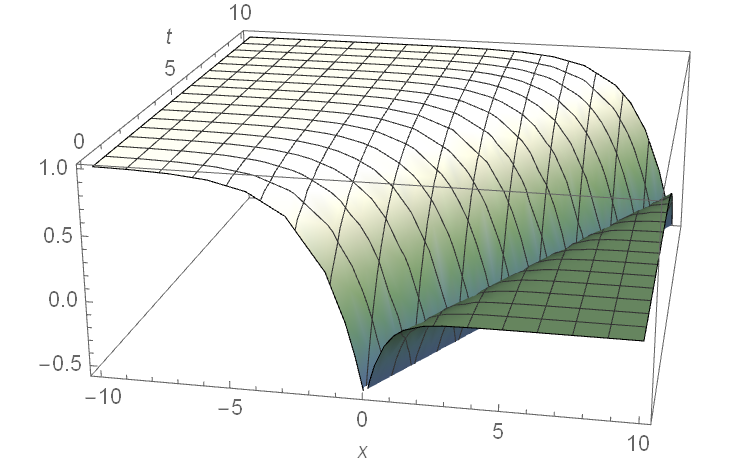
\includegraphics[width=\textwidth]{Part2Plots/e2}
        \caption{$\epsilon=2$}
        \label{fig:t0}
    \end{subfigure}
    \begin{subfigure}[h]{0.4\textwidth}
        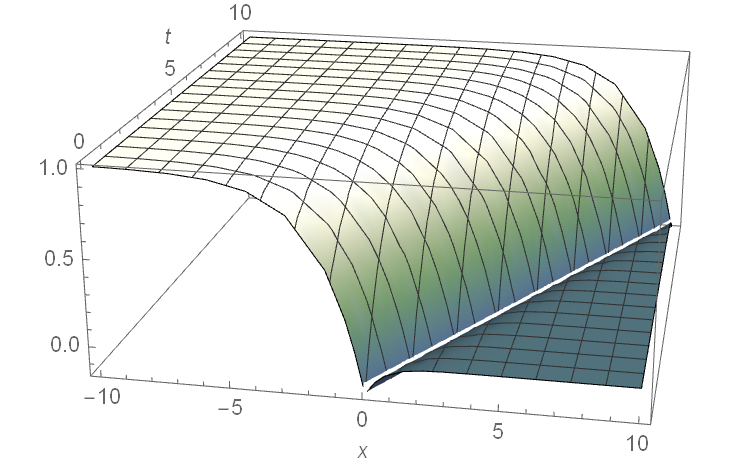
\includegraphics[width=\textwidth]{Part2Plots/e1}
        \caption{$\epsilon=1$}
        \label{fig:t1}
    \end{subfigure}
    \begin{subfigure}[h]{0.4\textwidth}
        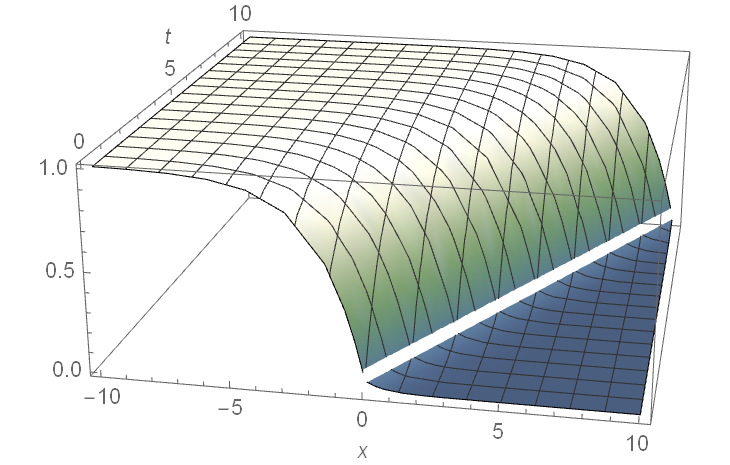
\includegraphics[width=\textwidth]{Part2Plots/e05}
        \caption{$\epsilon=0.5$}
        \label{fig:t10}
    \end{subfigure}
    \begin{subfigure}[h]{0.4\textwidth}
        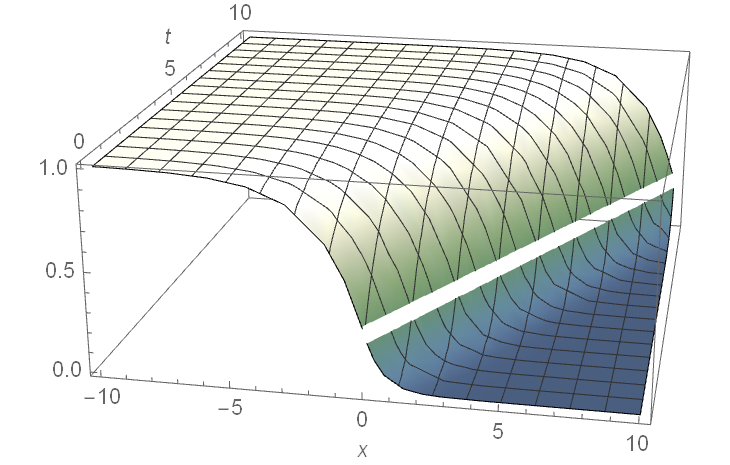
\includegraphics[width=\textwidth]{Part2Plots/e0}
        \caption{$\epsilon=0.01$}
        \label{fig:t100}
    \end{subfigure}
    \caption{$v(x,t) = V(\xi) + \epsilon V'(\xi)$ with various $\epsilon$ values}\label{fig:timeplots}
\end{figure}

\subsubsection{$\lambda > 0$ Case}
\begin{equation}\label{solnlambda+}
\psi_{\lambda >0}(\xi,t)=
\begin{cases}
\ \frac{-1}{\sqrt{c^2+4(\lambda+1)}}e^{\frac{-c+\sqrt{c^2+4(\lambda+1)}}{2}\xi},\quad \xi < 0 \\
\ \frac{-1}{\sqrt{c^2+4(\lambda+1)}}e^{\frac{-c-\sqrt{c^2+4(\lambda+1)}}{2}\xi},\quad \xi > 0\\
\end{cases}
\end{equation}

\subsubsection{$\lambda < 0$ Case}
\begin{equation}\label{solnlambda-}
\psi_{\lambda <0}(\xi,t)=
\begin{cases}
\ \frac{-1}{\sqrt{c^2-4(\lambda-1)}}e^{\frac{-c+\sqrt{c^2-4(\lambda-1)}}{2}\xi},\quad \xi < 0 \\
\ \frac{-1}{\sqrt{c^2-4(\lambda-1)}}e^{\frac{-c-\sqrt{c^2-4(\lambda-1)}}{2}\xi},\quad \xi > 0\\
\end{cases}
\end{equation}

\pagebreak

\begin{thebibliography}{9}

\bibitem{textbook}
Haberman, Richard.
\textit{Applied Partial Differential Equations with Fourier Series and Boundary Value Problems}.
Pearson.

\bibitem{greens}
Tara LaForce.
\textit{Green's Function Course Notes}. \\
\texttt{https://web.stanford.edu/class/energy281/GreensFunctions.pdf}

\bibitem{perturb}
University of California, Davis.
\textit{Linearizing Equations About Rest Points}. \\
\texttt{https://www.math.ucdavis.edu/~temple/MAT22C/LecturesMat22CW15/5-\\LinearizedEquationsAboutRestPoints-22C-W15.pdf}

\bibitem{fourier}
USPAS.
\textit{Table of Fourier Transform Pairs}. \\\texttt{http://uspas.fnal.gov/materials/11ODU/FourierTransformPairs.pdf}

\end{thebibliography}

\end{document}



